\documentclass[11pt]{article}

\usepackage{amsmath}
\usepackage{mathtools}
\usepackage{geometry}
\geometry{a4paper}
\usepackage[parfill]{parskip}
\usepackage{graphicx}
\usepackage{amssymb}
\usepackage{epstopdf}
\usepackage{listings}
\lstset{language = C++}
\usepackage{url}

\newcommand{\re}[1]{{{#1}_R}}
\newcommand{\im}[1]{{{#1}_I}}

\title{Power Flow Theory}
\author{Dan Gordon}
\date{}

\begin{document}
\maketitle

\section{Nomenclature}
\begin{align*}
y_{ik} &= g_{ik} + jb_{ik} = \text{complex admittance along branch $ik$.} \\
Y_{ik} &= G_{ik} + jB_{ik} = \text{nodal admittance matrix element $i, k$.} \\
&= 
	\begin{cases}
		-y_{ik}&\text{if $i \ne k$} \\
		y_i + \sum_l y_{il}& \text{if $i = k$}
	\end{cases} \\
V_i &= \text{complex voltage at bus $i$.} \\
M_i &= \text{voltage magnitude at bus $i$, $M_i := |V_i|$.} \\
I_{\text{br}i} &= \text{complex current injection from branches at bus $i$.} \\
I_{\text{ld}i} &= \text{total complex current injection from load at bus $i$.} \\
I_{\text{bus}i} &= \text{complex current injection due to the bus at bus $i$.} \\
S_{\text{bus}i} &= \text{complex power injection due to bus $i$.} \\
S_{ci} &= \text{constant power component of load at bus $i$.} \\
I_{ci} &= \text{constant current injection component of load.} \\
y_{ci} &= \text{constant impedance component of load.} \\
\delta_{ik} &= \text{the Kronecker delta, $\delta_{ik} = 1$ if $i = k$, 0 otherwise.}
\end{align*}

\section{Power flow equations in current form}
For simplicity, we write all bus quantities as injections \emph{into} the bus. Thus a normal load will use quantities expressed as negative injections, while a generator will have positive injections.

Each bus has an associated load, containing a constant power component, a constant current component, and a constant shunt impedance current. As well as receiving injections from branches and loads, busses provide their own injections according to their bus type. PQ busses provide a specified complex power injection. PV busses instead keep the voltage magnitude of the bus constant while providing a specified real power injection. Slack busses keep the complex voltage of the bus constant.

The total current injection into bus $i$ is:
\begin{align}
I_i &= I_{\text{br}, i} + I_{\text{ld}i} + I_{\text{bus}, i} = 0\\
I_{\text{bri}} &= -\sum_{k=0}^NY_{ik}V_k \\
I_{\text{ld}i} &= \frac{S^*_{ci}}{V^*_i} + I_{ci} - y_{ci}V_i \\
I_{\text{bus}i} &= \frac{S^*_{\text{bus}i}}{V^*_i}
\end{align}
which is zero, due to Kirchoff's current conservation law. Thus,
\begin{align}
I_i &= \frac{S^*_{ci} + S^*_{\text{bus}i}}{V^*_i} + I_{ci} - y_{ci}V_i - \sum_{k=0}^NY_{ik}V_k = 0
\end{align}
or, absorbing $y_c$ into $Y$ and $S_{\text{bus}}$ into $S_c$ we have
\begin{align}
I_i &= \frac{S'^*_{ci}}{V^*_i} + I_{ci} - \sum_{k=0}^NY'_{ik}V_k = 0
\end{align}
where
\begin{align}
	Y'_{ik} &= Y_{ik} + y_{ci}\delta_{ki}
\end{align}
and $S'_c = S_c + S_{\text{bus}}$.

Real and imaginary components are:
\begin{align}
\re{I}_i &= \frac{P'_{ci}\re{V}_{i} + Q'_{ci}\im{V}_{i}}{M^2_i} + \re{I_c}_{i} + \sum_{k=0}^N\left(-G'_{ik}\re{V}_k + B'_{ik}\im{V}_k\right) \\
\im{I}_i &= \frac{P'_{ci}\im{V}_{i} - Q'_{ci}\re{V}_{i}}{M^2_i} + \im{I_c}_{i} + \sum_{k=0}^N\left(-G'_{ik}\im{V}_k - B'_{ik}\re{V}_k\right) = 0
\end{align}

\subsection{Newton-Raphson equations}
For PQ busses, the unknowns are the real and imaginary parts of $V$, so this equation can be solved using the Newton-Raphson method. Letting the function to which we want to find the zero be $f = \{\re{I}, \im{I}\}$, the unknows be $x = \{\re{V}, \im{V}\}$, we wish to solve $f(x) = 0$. Using the Jacobian
\begin{align}
J_{ik}(x) = \frac{\partial f_i(x)}{\partial x_k}
\end{align}
the NR method calculates the update to $x$ at each iteration as the solution to the linear equations
\begin{align}
-f_{(n)} &= J(x_{(n)})(x_{(n+1)}-x_{(n)}) = J(x_{(n)})\Delta x_{(n,n+1)}
\end{align}
The Jacobian is given by:
\begin{align}
\frac{\partial \re{I}_i}{\partial \re{V}_{k}} &= \left[-\frac{2\re{V}_k(P'_{ck}\re{V}_k + Q'_{ck}\im{V}_k)}{M_k^4} + \frac{P'_{ck}}{M_k^2} \right]\delta_{ik} - G'_{ik} \\
\frac{\partial \re{I}_i}{\partial \im{V}_{k}} &= \left[-\frac{2\im{V}_k(P'_{ck}\re{V}_k + Q'_{ck}\im{V}_k)}{M_k^4} + \frac{Q'_{ck}}{M_k^2} \right]\delta_{ik}  + B'_{ik} \\
\frac{\partial \im{I}_i}{\partial \re{V}_{k}} &= \left[-\frac{2\re{V}_k(P'_{ck}\im{V}_k - Q'_{ck}\re{V}_k)}{M_k^4} - \frac{Q'_{ck}}{M_k^2} \right]\delta_{ik}  - B'_{ik} \\
\frac{\partial \im{I}_i}{\partial \im{V}_{k}} &= \left[-\frac{2\im{V}_k(P'_{ck}\im{V}_k - Q'_{ck}\re{V}_k)}{M_k^4} + \frac{P'_{ck}}{M_k^2} \right] \delta_{ik} - G'_{ik} \\
\end{align}

\subsection{PV busses}
For a PV bus $k$, the power flow equations also hold, but with $Q_{\text{bus}}$ being considered as a variable rather than a constant, and an extra constraint:
\begin{align}
\Delta M^2_k = \re{V}_{k}^2 + \im{V}_k^2 - M^2_{\text{PV}k} = 0
\end{align}

The corresponding rows in the NR equation may be solved by hand, with the following update:
\begin{align}
\re{\Delta V}_k &= \frac{M^2_{\text{PV}k} - \re{V}_k^2 - \im{V}_k^2- 2\im{V}_k\im{\Delta V}_k}{2\re{V}_k}
\end{align}
Thus, $\re{\Delta V}$ may be eliminated from the NR equations.  First write the Jacobian as if all busses were PQ. Let $k$ be a PV bus. Take the column corresponding to $\re{\Delta V}_k$, and add its product with $-\im{V}_k/\re{V}_k$ to the matching column for  $\im{\Delta V}_k$. Add its product with $(M^2_{\text{PV}k} - \re{V}_k^2 - \im{V}_k^2)/(2\re{V}_k)$ to $f$. The column and the corresponding element of $x$ will now be replaced to correspond to $Q_k$. Set the column to zero, and set the block diagonal elements, using:
\begin{align}
\frac{\partial \re{I}_k}{\partial Q_{\text{bus}k}} &= \frac{\im{V}_k}{M_k^2} \\
\frac{\partial \im{I}_k}{\partial Q_{\text{bus}k}} &= -\frac{\re{V}_k}{M_k^2}
\end{align}
\section{Multi phase lines}
Lines are typically handled in terms of $a$, $b$, $c$ and $d$ matrices. Assume for discussion that there are three phases, so these are $3 \times 3$ matrices, and $V$ and $I$ are assumed to be 3-vectors.
\begin{align}
	\begin{bmatrix} V_0 \\ I_0 \end{bmatrix} &=
	\begin{bmatrix} a & -b \\ c & -d \end{bmatrix} \begin{bmatrix} V_1 \\ I_1 \end{bmatrix}
\end{align}
Be careful of signs! Conventionally, the equations are written in terms of currents entering and leaving the line. But we'll move to a nodal admittance model, and hence all currents are treated as injections. This is why we have a negative sign on $b$ and $d$.

These equations can be transformed to the following:
\begin{align}
	\begin{bmatrix} I_0 \\ I_1 \end{bmatrix} &=
	\begin{bmatrix} db^{-1} & c - db^{-1}a \\ -b^{-1} & b^{-1}a \end{bmatrix} \begin{bmatrix} V_0 \\ V_1 \end{bmatrix} = Y\begin{bmatrix} V_0 \\ V_1 \end{bmatrix} 
\end{align}
which defines the nodal admittance matrix $Y$.

What is the interpretation of $a$, $b$, $c$, $d$? From Kersting \cite{KerstingXXXXa}, using a pi-model of a transmission line, $Z$ being the matrix of self and cross impedances of the line, $U$ being the identity matrix and $Y_s/2$ being the shunt admittance matrix for each of the two legs of the pi, we have
\begin{align}
a = d &= U + \frac{1}{2}ZY_s \\
b &= Z \\
c &= Y_s + \frac{1}{4}Y_s Z Y_s
\end{align}
and thus
\begin{align}
Y &= \begin{bmatrix} Z^{-1} + \frac{1}{2}ZY_sZ^{-1} & \frac{1}{2}Y_s + \frac{1}{2}Y_sZY_s - Z^{-1}-\frac{1}{2}ZY_sZ^{-1}-\frac{1}{4}ZY^2 \\
-Z^{-1} & Z^{-1}+\frac{1}{2}Y \end{bmatrix} 
\end{align}
\subsection{Short three wire lines}
For three phase delta lines of up to around 80 km in length, the shunt admittance $Y_s$ is small enough to neglect, and thus the nodal admittance matrix is:
\begin{align}
	Y &=
	\begin{bmatrix} Z^{-1} & -Z^{-1} \\ -Z^{-1} & Z^{-1} \end{bmatrix}
\end{align}
which is very reminiscent of the expression used in the single wire definition of nodal admittance.
\section{Transformers}
\subsection{Single phase transformers}
For an ideal transformer with a single turns ratio $r = n_0/n_1$, we have
\begin{align}
\begin{bmatrix}V_0 \\ I_0\end{bmatrix} &= \begin{bmatrix}n & 0 \\ 0 & -1/n\end{bmatrix}\begin{bmatrix}V_1 \\ I_1 \end{bmatrix}
\end{align}
This can't be modelled correctly in the formalism of nodal admittance.

A real transformer includes a leakage impedance (due to finite resistance of copper windings and core losses) and a shunt magnetising impedance. The latter is often large and may often be ignored. The nodal admittance matrix may be then derived:
\begin{align}
\begin{bmatrix}I_A \\ I_B \end{bmatrix} &= 
\begin{bmatrix}y_l/|a|^2 & -y_l/a^* \\ -y_l/a & y_l\end{bmatrix}
\begin{bmatrix}V_P \\ V_S \end{bmatrix}
\end{align}
where $a = V_P / V_S = N_P / N_S$ for an ideal transformer.

\subsection{Three-phase transformers}
The nodal admittance matrices of three-phase transformers may be derived from the single-phase expression, above, combined with information about the connections between phases.
\subsubsection{Delta-GWye}
\begin{figure}
\begin{center}
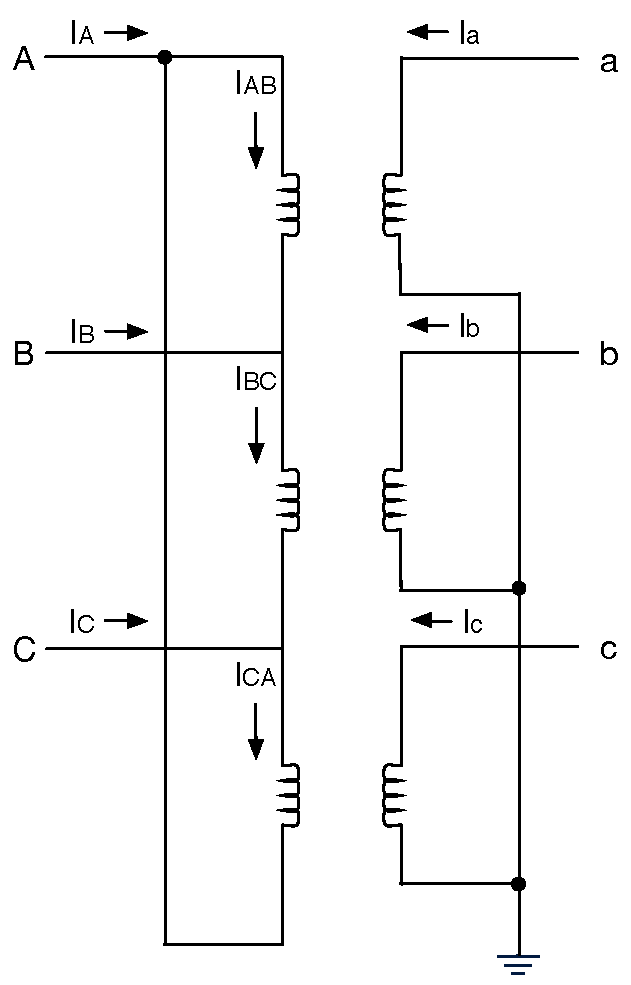
\includegraphics[width=7cm]{DeltaGWye.pdf}
\caption{Schematic of a Delta-GWye transformer}
\label{FIG_DELTA_GWYE}
\end{center}
\end{figure}
Considering Fig. \ref{FIG_DELTA_GWYE}, we have,
\begin{align}
I_{AB} &= \frac{y_l}{|a|^2}(V_A - V_B) - \frac{y_l}{a^*}V_a \\
I_{BC} &= \frac{y_l}{|a|^2}(V_B - V_C) - \frac{y_l}{a^*}V_b \\
I_{CA} &= \frac{y_l}{|a|^2}(V_C - V_A) - \frac{y_l}{a^*}V_c \\
I_a &= -\frac{y_l}{a}(V_A - V_B) + y_l V_a \\
I_b &= -\frac{y_l}{a}(V_B - V_C) + y_l V_b \\
I_c &= -\frac{y_l}{a}(V_C - V_A) + y_l V_c \\
\end{align}
Also, by the KCL, we have
\begin{align}
I_A &= I_{AB} - I_{CA} \\
&= \frac{y_l}{|a|^2}(2V_A - V_B - V_C) + \frac{y_l}{a^*}(V_c - V_a) \\
I_B &= I_{BC} - I_{AB} \\
&= \frac{y_l}{|a|^2}(2V_B - V_C - V_A) + \frac{y_l}{a^*}(V_a - V_b) \\
I_C &= I_{CA} - I_{BC} \\
&= \frac{y_l}{|a|^2}(2V_C - V_A - V_B) + \frac{y_l}{a^*}(V_b - V_c)
\end{align}
So we can immediately write down the nodal admittance relationship:
\begin{align}
\begin{bmatrix}I_A \\ I_B \\ I_C \\ I_a \\ I_b \\ I_c\end{bmatrix} &=
y_l \begin{bmatrix}
	2/|a|^2 & -1/|a|^2 & -1/|a|^2 & -1/a^* & 0 & 1/a^* \\
	-1/|a|^2 & 2/|a|^2 &  -1/|a|^2 & 1/a^*  & -1/a^* & 0 \\
	-1/|a|^2 &  -1/|a|^2 & 2/|a|^2 & 0 & 1/a^*  & -1/a^* \\
	-1/a & 1/a & 0 & 1 & 0 & 0 \\
	0 & -1/a & 1/a & 0 & 1 & 0 \\
	1/a & 0 & -1/a & 0 & 0 & 1
\end{bmatrix}
\begin{bmatrix}V_A \\ V_B \\ V_C \\ V_a \\ V_b \\ V_c\end{bmatrix}
\end{align}
with the nodal admittance matrix being specified by the matrix on the right, including the factor of $y_l$.
\end{document}